% Copyright 2024 by Marcos Laureano (marcos.laureano@ifpr.edu.br)
% This file may be distributed and/or modified
%
% 1. under the LaTeX Project Public License and/or
% 2. under the GNU Public License.

\documentclass[varwidth]{standalone}
\usepackage{caption}
\usepackage{subcaption}
\usepackage{pgfplots}
    \usepackage{adjustbox}
\pgfplotsset{compat=newest}
\usetikzlibrary{positioning, backgrounds}
\begin{document}
        
        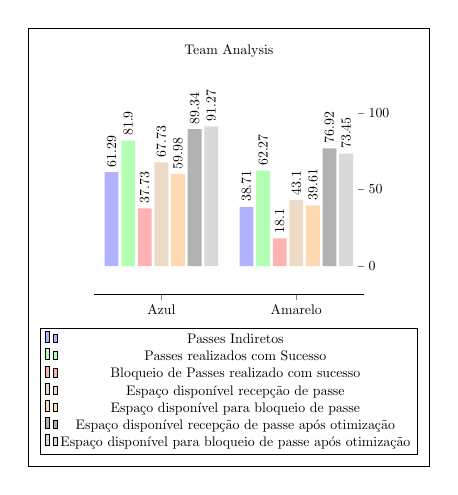
\begin{tikzpicture}[scale=.5,framed]
        \centering
        \begin{axis}[legend columns=1,
        ymajorgrids, tick align=inside,
        major grid style={draw=white},
        enlarge y limits={value=0,upper},
        axis x line*=bottom,
        axis y line*=right,
        y axis line style={opacity=0},
        enlarge x limits=true, scale=1,
        ybar,
        enlargelimits=.5,
        legend style={at={(0.5,-0.15)},
            anchor=north,legend columns=-1},
        symbolic x coords={Azul, Amarelo},
        xtick=data,
        every node near coord/.append style={rotate=90, anchor=west},
        nodes near coords,
        nodes near coords align={vertical},bar width=10pt,title=Team Analysis,
        ]
        \addplot [draw=none, fill=blue!30] coordinates {
            (Azul,61.29)
            (Amarelo,38.71) 
        };
        
        \addplot [draw=none, fill=green!30] coordinates {
            (Azul,81.90)
            (Amarelo,62.27) 
        };        
        
        \addplot [draw=none, fill=red!30] coordinates {
            (Azul,37.73)
            (Amarelo,18.1) 
        }; 
        
        \addplot [draw=none, fill=brown!30] coordinates {
            (Azul,67.73)
            (Amarelo,43.1) 
        }; 
        
        \addplot [draw=none, fill=orange!30] coordinates {
            (Azul,59.98)
            (Amarelo,39.61) 
        }; 
        
        \addplot [draw=none, fill=black!30] coordinates {
            (Azul,89.34)
            (Amarelo,76.92) 
        }; 
        
        \addplot [draw=none, fill=gray!30] coordinates {
            (Azul,91.27)
            (Amarelo,73.45) 
        }; 
        
        \legend{Passes Indiretos, Passes realizados com Sucesso, Bloqueio de Passes realizado com sucesso, Espaço disponível recepção de passe,
            Espaço disponível para bloqueio de passe, Espaço disponível recepção de passe após otimização, Espaço disponível para bloqueio de passe após otimização}
        \end{axis}
        \end{tikzpicture}
\end{document}